\documentclass{article}\usepackage[]{graphicx}\usepackage[]{color}
%% maxwidth is the original width if it is less than linewidth
%% otherwise use linewidth (to make sure the graphics do not exceed the margin)
\makeatletter
\def\maxwidth{ %
  \ifdim\Gin@nat@width>\linewidth
    \linewidth
  \else
    \Gin@nat@width
  \fi
}
\makeatother

\definecolor{fgcolor}{rgb}{0.345, 0.345, 0.345}
\newcommand{\hlnum}[1]{\textcolor[rgb]{0.686,0.059,0.569}{#1}}%
\newcommand{\hlstr}[1]{\textcolor[rgb]{0.192,0.494,0.8}{#1}}%
\newcommand{\hlcom}[1]{\textcolor[rgb]{0.678,0.584,0.686}{\textit{#1}}}%
\newcommand{\hlopt}[1]{\textcolor[rgb]{0,0,0}{#1}}%
\newcommand{\hlstd}[1]{\textcolor[rgb]{0.345,0.345,0.345}{#1}}%
\newcommand{\hlkwa}[1]{\textcolor[rgb]{0.161,0.373,0.58}{\textbf{#1}}}%
\newcommand{\hlkwb}[1]{\textcolor[rgb]{0.69,0.353,0.396}{#1}}%
\newcommand{\hlkwc}[1]{\textcolor[rgb]{0.333,0.667,0.333}{#1}}%
\newcommand{\hlkwd}[1]{\textcolor[rgb]{0.737,0.353,0.396}{\textbf{#1}}}%

\usepackage{framed}
\makeatletter
\newenvironment{kframe}{%
 \def\at@end@of@kframe{}%
 \ifinner\ifhmode%
  \def\at@end@of@kframe{\end{minipage}}%
  \begin{minipage}{\columnwidth}%
 \fi\fi%
 \def\FrameCommand##1{\hskip\@totalleftmargin \hskip-\fboxsep
 \colorbox{shadecolor}{##1}\hskip-\fboxsep
     % There is no \\@totalrightmargin, so:
     \hskip-\linewidth \hskip-\@totalleftmargin \hskip\columnwidth}%
 \MakeFramed {\advance\hsize-\width
   \@totalleftmargin\z@ \linewidth\hsize
   \@setminipage}}%
 {\par\unskip\endMakeFramed%
 \at@end@of@kframe}
\makeatother

\definecolor{shadecolor}{rgb}{.97, .97, .97}
\definecolor{messagecolor}{rgb}{0, 0, 0}
\definecolor{warningcolor}{rgb}{1, 0, 1}
\definecolor{errorcolor}{rgb}{1, 0, 0}
\newenvironment{knitrout}{}{} % an empty environment to be redefined in TeX

\usepackage{alltt}
\usepackage[inner=2cm,outer=2cm]{geometry}
\usepackage{hyperref}
\hypersetup{colorlinks=true}
\usepackage{dashrule}
\usepackage{authblk}
\usepackage{csquotes}
\usepackage{tikz}
\usepackage{framed}
\usepackage{color}
%\newenvironment{shadequote}%
%{\begin{snugshade}\begin{quote}}
%{\hfill\end{quote}\end{snugshade}}

%\definecolor{shadecolor}{rgb}{0.9,0.9,0.9}
\IfFileExists{upquote.sty}{\usepackage{upquote}}{}
\begin{document}

\title{TDM}
\author{Jeffrey A. Thompson}
\affil{Greene Lab, Geisel School of Medicine, Dartmouth College}
\maketitle

% !Rnw weave = knitr 
%\VignetteEngine{knitr::knitr}
%\VignetteIndexEntry{AnnotationParser}



\section{Training Distribution Matching}

To perform the TDM transformation you need to have a reference dataset and a
target dataset. The reference dataset should be from microarray expression
experiments and the target dataset should be from RNA-seq. The target dataset
will be transformed to have similar characteristics to the reference.

As an example, the TDM package contains some sample data. These data can be
loaded as follows:

\begin{knitrout}
\definecolor{shadecolor}{rgb}{0.969, 0.969, 0.969}\color{fgcolor}\begin{kframe}
\begin{alltt}
\hlkwd{data}\hlstd{(meta)}
\hlkwd{data}\hlstd{(tcga)}
\end{alltt}
\end{kframe}
\end{knitrout}

The data are loaded into variables \textbf{meta} and \textbf{tcga}. Here is a
summary of their characteristics:

\begin{knitrout}
\definecolor{shadecolor}{rgb}{0.969, 0.969, 0.969}\color{fgcolor}\begin{kframe}
\begin{alltt}
\hlkwd{summary}\hlstd{(}\hlkwd{as.vector}\hlstd{(}\hlkwd{as.matrix}\hlstd{(meta)))}
\end{alltt}
\begin{verbatim}
##    Min. 1st Qu.  Median    Mean 3rd Qu.    Max. 
##   4.776   6.804   7.774   8.006   8.966  14.880
\end{verbatim}
\begin{alltt}
\hlkwd{summary}\hlstd{(}\hlkwd{as.vector}\hlstd{(}\hlkwd{as.matrix}\hlstd{(tcga)))}
\end{alltt}
\begin{verbatim}
##      Min.   1st Qu.    Median      Mean   3rd Qu.      Max. 
##       0.0     184.8     613.6    2143.0    1702.0 2066000.0
\end{verbatim}
\end{kframe}
\end{knitrout}

If we simply scaled the TCGA data to be in the same range, the distribution
would be quite different:

\begin{knitrout}
\definecolor{shadecolor}{rgb}{0.969, 0.969, 0.969}\color{fgcolor}\begin{kframe}
\begin{alltt}
\hlkwd{load_it}\hlstd{(}\hlstr{"scales"}\hlstd{)}
\hlstd{tcga_vec} \hlkwb{=} \hlkwd{rescale}\hlstd{(}\hlkwd{as.vector}\hlstd{(}\hlkwd{as.matrix}\hlstd{(tcga)),} \hlkwc{to}\hlstd{=}\hlkwd{c}\hlstd{(}\hlkwd{min}\hlstd{(meta),} \hlkwd{max}\hlstd{(meta)))}
\hlkwd{summary}\hlstd{(tcga_vec)}
\end{alltt}
\begin{verbatim}
##    Min. 1st Qu.  Median    Mean 3rd Qu.    Max. 
##   4.776   4.776   4.779   4.786   4.784  14.880
\end{verbatim}
\end{kframe}
\end{knitrout}

One might try log transforming the RNA-seq data, but this also is
unsatisfactory:

\begin{knitrout}
\definecolor{shadecolor}{rgb}{0.969, 0.969, 0.969}\color{fgcolor}\begin{kframe}
\begin{alltt}
\hlkwd{load_it}\hlstd{(}\hlstr{"data.table"}\hlstd{)}
\hlstd{tcga_log} \hlkwb{=} \hlkwd{log_transform_p1}\hlstd{(}\hlkwd{data.table}\hlstd{(}\hlkwd{cbind}\hlstd{(}\hlkwc{gene}\hlstd{=}\hlkwd{rownames}\hlstd{(tcga), tcga)))}
\hlkwd{summary}\hlstd{(}\hlkwd{as.vector}\hlstd{(}\hlkwd{data.matrix}\hlstd{(tcga_log[,}\hlnum{2}\hlopt{:}\hlkwd{ncol}\hlstd{(tcga_log),}\hlkwc{with}\hlstd{=F])))}
\end{alltt}
\begin{verbatim}
##    Min. 1st Qu.  Median    Mean 3rd Qu.    Max. 
##   0.000   7.537   9.263   8.999  10.730  20.980
\end{verbatim}
\end{kframe}
\end{knitrout}

If we TDM transform the data, the results appear to be much improved:

\begin{knitrout}
\definecolor{shadecolor}{rgb}{0.969, 0.969, 0.969}\color{fgcolor}\begin{kframe}
\begin{alltt}
\hlstd{tcga_tdm} \hlkwb{=} \hlkwd{tdm_transform}\hlstd{(}\hlkwc{ref_data} \hlstd{=} \hlkwd{data.table}\hlstd{(}\hlkwd{cbind}\hlstd{(}\hlkwc{gene}\hlstd{=}\hlkwd{rownames}\hlstd{(meta), meta)),}
\hlkwc{target_data} \hlstd{=} \hlkwd{data.table}\hlstd{(}\hlkwd{cbind}\hlstd{(}\hlkwc{gene}\hlstd{=}\hlkwd{rownames}\hlstd{(tcga), tcga)))}
\hlkwd{summary}\hlstd{(}\hlkwd{as.vector}\hlstd{(}\hlkwd{data.matrix}\hlstd{(tcga_tdm[,}\hlnum{2}\hlopt{:}\hlkwd{ncol}\hlstd{(tcga_tdm),}\hlkwc{with}\hlstd{=F])))}
\end{alltt}
\begin{verbatim}
##    Min. 1st Qu.  Median    Mean 3rd Qu.    Max. 
##   4.776   5.766   7.338   7.448   8.793  14.880
\end{verbatim}
\end{kframe}
\end{knitrout}

Finally, here is a plot comparing the distributions of the reference data, the
scaled data, the log transformed data, and the TDM transformed data:



\begin{figure}
  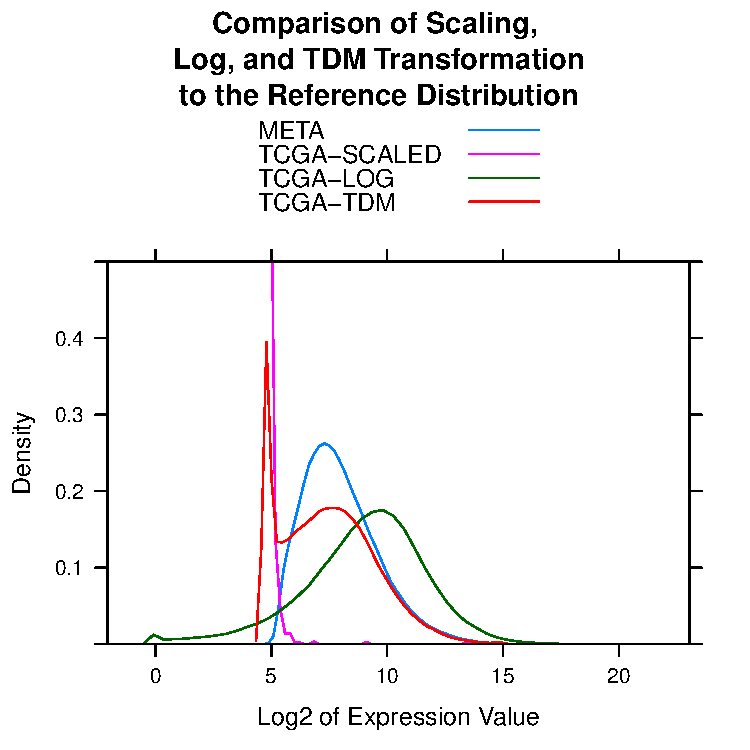
\includegraphics{figures/comparison-1}
  \label{fig:comparison}
  \caption{TDM brings the sample RNA-seq data closest to the reference distribution. Log2 transformation creates a left-skewed distribution that is not typical of microarray data, making comparison between the datasets difficult, while simple scaling creates a right-skewed distribution.}
\end{figure}

\end{document}
